\documentclass{article}
\usepackage[utf8]{inputenc}
\usepackage{hyperref}
\usepackage[letterpaper, portrait, margin=1in]{geometry}
\usepackage{enumitem}
\usepackage{amsmath}
\usepackage{booktabs}
\usepackage{graphicx}
\usepackage{longtable}

\usepackage{hyperref}
\hypersetup{
colorlinks=true,
    linkcolor=black,
    filecolor=black,      
    urlcolor=blue,
    citecolor=black,
}
\usepackage{natbib}

\usepackage{titlesec}
  
\title{ECON 7103 Homework 4}
\author{Yifan Liu (yliu3494)}
\date{Spring 2023}
  
\begin{document}
  
\maketitle



\noindent
\section{Python}
\noindent\rule{17cm}{0.4pt}
1. Visualization of the parallel trends
\begin{figure}[h]
    \centering
    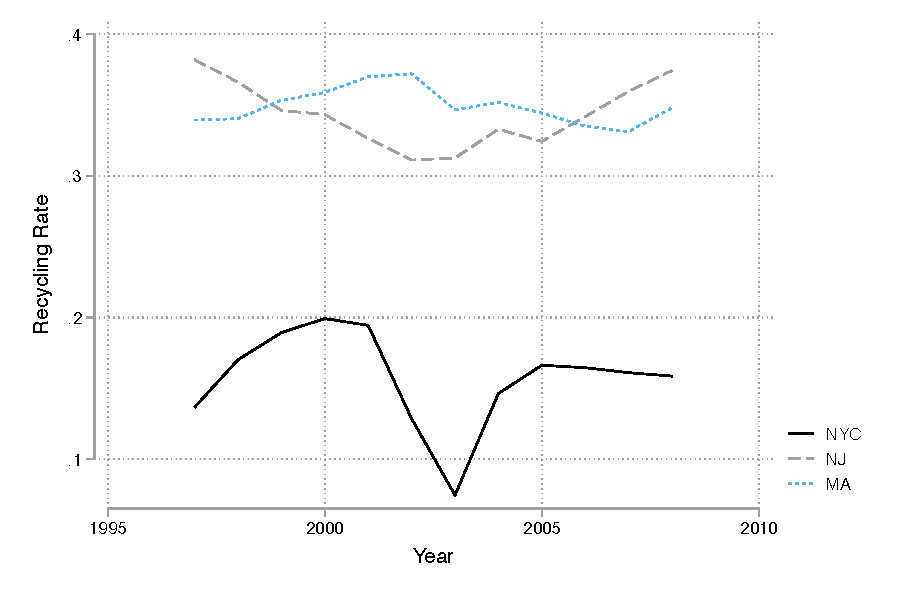
\includegraphics[scale = 0.7]{Q1.pdf}
    \caption{Bycatch before and after treatment for treated and control groups in months of 2017 and 2018}
    \label{fig:Q1}
\end{figure}
\\
From Figure 1, we can tell that there are parallel trends before treatment (January 2018) between treatment and control groups. 
\bigskip
\\
2. DID
\bigskip
\\
$DID = \{E[Y_{igt}| g(i) = treat, t= Post] - E[Y_{igt}| g(i) = treat, t= Pre]\} - \{E[Y_{igt}| g(i) = control, t= Post] - E[Y_{igt}| g(i) = control, t= Pre]\}$
\smallskip
\\
= (139612.51 - 148430.64) - (138001.81 - 137228.6)
\smallskip
\\
= -9591.35
\smallskip
\\
The DID estimator is defined as the difference in average monthly yields of bycatch in the treatment group before and after treatment minus the difference in average monthly yields of bycatch in the control group before and after treatment.
\\
The intuition of the estimator here is the effect of the program  on the monthly yields of bycatch. The program was implemented by an environmental nonprofit to reduce bycatch. 
\bigskip
\\
3. 
\bigskip
\\
(a)
\smallskip
\\
Table 1 shows the two-period difference-in-differences estimator using the regression specification in the equation (3) and the observations in December 2017 and January 2018 only.
\begin{table}[h]
    \centering
    \begin{center}
\begin{tabular}{lclc}
\toprule
\textbf{Dep. Variable:}    &     bycatch      & \textbf{  R-squared:         } &     0.003   \\
\textbf{Model:}            &       OLS        & \textbf{  Adj. R-squared:    } &    -0.028   \\
\textbf{Method:}           &  Least Squares   & \textbf{  F-statistic:       } &     3.161   \\
\textbf{Date:}             & Sun, 12 Feb 2023 & \textbf{  Prob (F-statistic):} &   0.0327    \\
\textbf{Time:}             &     17:30:18     & \textbf{  Log-Likelihood:    } &   -1270.4   \\
\textbf{No. Observations:} &         100      & \textbf{  AIC:               } &     2549.   \\
\textbf{Df Residuals:}     &          96      & \textbf{  BIC:               } &     2559.   \\
\textbf{Df Model:}         &           3      & \textbf{                     } &             \\
\textbf{Covariance Type:}  &     cluster      & \textbf{                     } &             \\
\bottomrule
\end{tabular}
\begin{tabular}{lcccccc}
                      & \textbf{coef} & \textbf{std err} & \textbf{z} & \textbf{P$> |$z$|$} & \textbf{[0.025} & \textbf{0.975]}  \\
\midrule
\textbf{const}        &     1.38e+05  &     1.87e+04     &     7.396  &         0.000        &     1.01e+05    &     1.75e+05     \\
\textbf{pre}          &    -773.2158  &      598.685     &    -1.292  &         0.197        &    -1946.617    &      400.186     \\
\textbf{treated}      &     1.12e+04  &     2.35e+04     &     0.477  &         0.634        &    -3.49e+04    &     5.73e+04     \\
\textbf{treated:post} &   -9591.3495  &     3231.787     &    -2.968  &         0.003        &    -1.59e+04    &    -3257.164     \\
\bottomrule
\end{tabular}
\begin{tabular}{lclc}
\textbf{Omnibus:}       & 11.020 & \textbf{  Durbin-Watson:     } &    2.387  \\
\textbf{Prob(Omnibus):} &  0.004 & \textbf{  Jarque-Bera (JB):  } &   11.533  \\
\textbf{Skew:}          &  0.697 & \textbf{  Prob(JB):          } &  0.00313  \\
\textbf{Kurtosis:}      &  3.908 & \textbf{  Cond. No.          } &     6.89  \\
\bottomrule
\end{tabular}
%\caption{OLS Regression Results}
\end{center}

Notes: \newline
 [1] Standard Errors are robust to cluster correlation (cluster)
    \caption{Two-period difference-in-differences estimator using the regression specification in the equation (3)}
    \label{tab:Q3_a}
\end{table}
\bigskip
\\
(b)
\smallskip
\\
Table 2 shows the treatment estimator using the regression specification in the equation (4) and the full monthly sample.
\\
I deleted the month 13 to avoid multicollinearity. 
\\
Using the full monthly sample, the estimate of the treatment effects becomes smaller than the result with the observations in December 2017 and January 2018. 
\begin{table}[h]
    \centering
    \begin{center}
\begin{tabular}{lclc}
\toprule
\textbf{Dep. Variable:}    &     bycatch      & \textbf{  R-squared:         } &     0.003   \\
\textbf{Model:}            &       OLS        & \textbf{  Adj. R-squared:    } &    -0.018   \\
\textbf{Method:}           &  Least Squares   & \textbf{  F-statistic:       } &     7.349   \\
\textbf{Date:}             & Mon, 13 Feb 2023 & \textbf{  Prob (F-statistic):} &  1.74e-09   \\
\textbf{Time:}             &     20:23:01     & \textbf{  Log-Likelihood:    } &   -15242.   \\
\textbf{No. Observations:} &        1200      & \textbf{  AIC:               } & 3.054e+04   \\
\textbf{Df Residuals:}     &        1174      & \textbf{  BIC:               } & 3.067e+04   \\
\textbf{Df Model:}         &          25      & \textbf{                     } &             \\
\textbf{Covariance Type:}  &     cluster      & \textbf{                     } &             \\
\bottomrule
\end{tabular}
\begin{tabular}{lcccccc}
                      & \textbf{coef} & \textbf{std err} & \textbf{z} & \textbf{P$> |$z$|$} & \textbf{[0.025} & \textbf{0.975]}  \\
\midrule
\textbf{const}        &    1.377e+05  &     1.86e+04     &     7.401  &         0.000        &     1.01e+05    &     1.74e+05     \\
\textbf{treated}      &    1.105e+04  &     2.32e+04     &     0.477  &         0.633        &    -3.43e+04    &     5.65e+04     \\
\textbf{treated:post} &   -8956.7837  &     3166.921     &    -2.828  &         0.005        &    -1.52e+04    &    -2749.732     \\
\textbf{month\_1}     &   -1585.8815  &      539.636     &    -2.939  &         0.003        &    -2643.549    &     -528.214     \\
\textbf{month\_2}     &   -1843.1931  &      500.218     &    -3.685  &         0.000        &    -2823.603    &     -862.783     \\
\textbf{month\_3}     &   -1524.8250  &      514.584     &    -2.963  &         0.003        &    -2533.392    &     -516.258     \\
\textbf{month\_4}     &   -1667.3508  &      516.646     &    -3.227  &         0.001        &    -2679.958    &     -654.743     \\
\textbf{month\_5}     &   -1941.1701  &      556.739     &    -3.487  &         0.000        &    -3032.359    &     -849.981     \\
\textbf{month\_6}     &   -1359.7701  &      592.424     &    -2.295  &         0.022        &    -2520.900    &     -198.640     \\
\textbf{month\_7}     &   -2007.1326  &      691.661     &    -2.902  &         0.004        &    -3362.764    &     -651.501     \\
\textbf{month\_8}     &   -1701.7864  &      567.648     &    -2.998  &         0.003        &    -2814.356    &     -589.217     \\
\textbf{month\_9}     &   -1726.8567  &      584.867     &    -2.953  &         0.003        &    -2873.175    &     -580.538     \\
\textbf{month\_10}    &    -945.9439  &      559.874     &    -1.690  &         0.091        &    -2043.276    &      151.388     \\
\textbf{month\_11}    &    -422.6513  &      555.809     &    -0.760  &         0.447        &    -1512.018    &      666.715     \\
\textbf{month\_12}    &    -430.5503  &      480.193     &    -0.897  &         0.370        &    -1371.711    &      510.610     \\
\textbf{month\_14}    &     517.6268  &      513.551     &     1.008  &         0.313        &     -488.915    &     1524.168     \\
\textbf{month\_15}    &     464.9736  &      477.082     &     0.975  &         0.330        &     -470.089    &     1400.036     \\
\textbf{month\_16}    &     833.5673  &      571.850     &     1.458  &         0.145        &     -287.238    &     1954.373     \\
\textbf{month\_17}    &    1151.7560  &      445.231     &     2.587  &         0.010        &      279.119    &     2024.392     \\
\textbf{month\_18}    &     707.9408  &      401.926     &     1.761  &         0.078        &      -79.819    &     1495.701     \\
\textbf{month\_19}    &     998.7330  &      453.848     &     2.201  &         0.028        &      109.208    &     1888.258     \\
\textbf{month\_20}    &    1178.5464  &      410.169     &     2.873  &         0.004        &      374.630    &     1982.463     \\
\textbf{month\_21}    &    1295.0004  &      369.765     &     3.502  &         0.000        &      570.275    &     2019.726     \\
\textbf{month\_22}    &    2000.9103  &      477.260     &     4.192  &         0.000        &     1065.498    &     2936.323     \\
\textbf{month\_23}    &    2157.1445  &      441.289     &     4.888  &         0.000        &     1292.233    &     3022.056     \\
\textbf{month\_24}    &    2293.5956  &      385.532     &     5.949  &         0.000        &     1537.967    &     3049.224     \\
\bottomrule
\end{tabular}
\begin{tabular}{lclc}
\textbf{Omnibus:}       & 95.036 & \textbf{  Durbin-Watson:     } &    2.431  \\
\textbf{Prob(Omnibus):} &  0.000 & \textbf{  Jarque-Bera (JB):  } &  124.308  \\
\textbf{Skew:}          &  0.670 & \textbf{  Prob(JB):          } & 1.02e-27  \\
\textbf{Kurtosis:}      &  3.832 & \textbf{  Cond. No.          } &     30.9  \\
\bottomrule
\end{tabular}
%\caption{OLS Regression Results}
\end{center}

Notes: \newline
 [1] Standard Errors are robust to cluster correlation (cluster)
    \caption{The treatment estimator using the regression specification in the equation (4)}
    \label{tab:Q3_b}
\end{table}
\bigskip
\\
(c)
\smallskip
\\
Table 3 shows the treatment estimator using the regression specification in the equation (5) with added controls and the full monthly sample.
\\ The estimate of the treatment effects becomes a bit smaller after adding controls.
\begin{table}[h]
    \centering
    \begin{center}
\begin{tabular}{lclc}
\toprule
\textbf{Dep. Variable:}    &     bycatch      & \textbf{  R-squared:         } &     0.991   \\
\textbf{Model:}            &       OLS        & \textbf{  Adj. R-squared:    } &     0.991   \\
\textbf{Method:}           &  Least Squares   & \textbf{  F-statistic:       } &     4733.   \\
\textbf{Date:}             & Mon, 13 Feb 2023 & \textbf{  Prob (F-statistic):} &  3.57e-75   \\
\textbf{Time:}             &     20:23:01     & \textbf{  Log-Likelihood:    } &   -12401.   \\
\textbf{No. Observations:} &        1200      & \textbf{  AIC:               } & 2.486e+04   \\
\textbf{Df Residuals:}     &        1171      & \textbf{  BIC:               } & 2.501e+04   \\
\textbf{Df Model:}         &          28      & \textbf{                     } &             \\
\textbf{Covariance Type:}  &     cluster      & \textbf{                     } &             \\
\bottomrule
\end{tabular}
\begin{tabular}{lcccccc}
                      & \textbf{coef} & \textbf{std err} & \textbf{z} & \textbf{P$> |$z$|$} & \textbf{[0.025} & \textbf{0.975]}  \\
\midrule
\textbf{const}        &    1424.1693  &     1176.857     &     1.210  &         0.226        &     -882.428    &     3730.767     \\
\textbf{treated}      &     -21.9017  &      308.244     &    -0.071  &         0.943        &     -626.049    &      582.246     \\
\textbf{firmsize}     &   -2119.7133  &     3406.960     &    -0.622  &         0.534        &    -8797.232    &     4557.805     \\
\textbf{shrimp}       &       1.0554  &        0.053     &    19.991  &         0.000        &        0.952    &        1.159     \\
\textbf{salmon}       &       0.6021  &        0.210     &     2.871  &         0.004        &        0.191    &        1.013     \\
\textbf{treated:post} &   -8436.2817  &     2823.973     &    -2.987  &         0.003        &     -1.4e+04    &    -2901.397     \\
\textbf{month\_1}     &     122.8366  &      285.466     &     0.430  &         0.667        &     -436.666    &      682.339     \\
\textbf{month\_2}     &     138.6053  &      289.076     &     0.479  &         0.632        &     -427.973    &      705.183     \\
\textbf{month\_3}     &     107.4263  &      253.662     &     0.424  &         0.672        &     -389.742    &      604.594     \\
\textbf{month\_4}     &     111.6298  &      232.909     &     0.479  &         0.632        &     -344.863    &      568.122     \\
\textbf{month\_5}     &     118.7962  &      225.810     &     0.526  &         0.599        &     -323.784    &      561.377     \\
\textbf{month\_6}     &      67.0887  &      166.699     &     0.402  &         0.687        &     -259.635    &      393.812     \\
\textbf{month\_7}     &     104.8093  &      189.877     &     0.552  &         0.581        &     -267.343    &      476.962     \\
\textbf{month\_8}     &      67.2376  &      136.640     &     0.492  &         0.623        &     -200.571    &      335.046     \\
\textbf{month\_9}     &      63.9654  &      131.159     &     0.488  &         0.626        &     -193.102    &      321.033     \\
\textbf{month\_10}    &      22.4845  &      100.222     &     0.224  &         0.822        &     -173.947    &      218.916     \\
\textbf{month\_11}    &     -16.6447  &       54.718     &    -0.304  &         0.761        &     -123.889    &       90.600     \\
\textbf{month\_12}    &     -20.9227  &       48.266     &    -0.433  &         0.665        &     -115.523    &       73.677     \\
\textbf{month\_14}    &     -65.7937  &       63.417     &    -1.037  &         0.300        &     -190.089    &       58.501     \\
\textbf{month\_15}    &     -35.9279  &       78.513     &    -0.458  &         0.647        &     -189.810    &      117.954     \\
\textbf{month\_16}    &    -128.3744  &       87.097     &    -1.474  &         0.141        &     -299.082    &       42.333     \\
\textbf{month\_17}    &    -142.7108  &      116.243     &    -1.228  &         0.220        &     -370.543    &       85.121     \\
\textbf{month\_18}    &     -64.5680  &      118.037     &    -0.547  &         0.584        &     -295.915    &      166.779     \\
\textbf{month\_19}    &    -148.3208  &      146.065     &    -1.015  &         0.310        &     -434.603    &      137.962     \\
\textbf{month\_20}    &    -193.6003  &      175.165     &    -1.105  &         0.269        &     -536.917    &      149.717     \\
\textbf{month\_21}    &    -162.2639  &      187.038     &    -0.868  &         0.386        &     -528.852    &      204.325     \\
\textbf{month\_22}    &    -254.3110  &      268.104     &    -0.949  &         0.343        &     -779.785    &      271.163     \\
\textbf{month\_23}    &    -326.6586  &      280.257     &    -1.166  &         0.244        &     -875.952    &      222.635     \\
\textbf{month\_24}    &    -285.8655  &      257.347     &    -1.111  &         0.267        &     -790.257    &      218.526     \\
\bottomrule
\end{tabular}
\begin{tabular}{lclc}
\textbf{Omnibus:}       & 717.103 & \textbf{  Durbin-Watson:     } &    1.297  \\
\textbf{Prob(Omnibus):} &   0.000 & \textbf{  Jarque-Bera (JB):  } & 6623.424  \\
\textbf{Skew:}          &  -2.679 & \textbf{  Prob(JB):          } &     0.00  \\
\textbf{Kurtosis:}      &  13.186 & \textbf{  Cond. No.          } & 4.57e+06  \\
\bottomrule
\end{tabular}
%\caption{OLS Regression Results}
\end{center}

Notes: \newline
 [1] Standard Errors are robust to cluster correlation (cluster) \newline
 [2] The condition number is large, 4.57e+06. This might indicate that there are \newline
 strong multicollinearity or other numerical problems.
    \caption{The treatment estimator using the regression specification in the equation (5)}
    \label{tab:Q3_c}
\end{table}
\bigskip
\\
(d)
\smallskip
\\
Table 4 reports the results from the previous three questions (a) (b) (c) in a table with clustered standard errors at the firm level. Note that here we omit the estimates of the coefficients on the month and firm indicators in the table. 
\smallskip
\\
The result in the model (a) is the same with my previous calculation in the question 2. The estimator is smaller in the model (b). This means the treatment effect of the program is smaller while using the full monthly sample. The estimator in the model (c) is a bit smaller than that in the model (b) due to the addition of control variables. The lack of these controls can make the treatment effect of the program biased upward. After controlling for firm size and other covariates that change over time, the estimator becomes slightly smaller.  
\begin{table}[h]
    \centering
    \begin{tabular}{llll}
\toprule
{} & \multicolumn{3}{l}{Estimates} \\
{} & \multicolumn{3}{l}{(clustered s.d.)} \\
{} &              (a) &         (b) &        (c) \\
\midrule
Treatment group(gamma)         &         11202.04 &    11052.45 &   -2119.71 \\
                               &        (23502.9) &  (23162.97) &  (3406.96) \\
When a firm is treated (delta) &         -9591.35 &    -8956.78 &   -8436.28 \\
                               &        (3231.79) &   (3166.92) &  (2823.97) \\
Constant                       &        138001.81 &   137739.93 &    1424.17 \\
                               &        (18657.8) &  (18611.19) &  (1176.86) \\
Observations                   &              100 &        1200 &       1200 \\
\bottomrule
\end{tabular}

    \caption{The treatment estimators using the regression specification in the equation (3)(4)(5)}
    \label{tab:Q3_d}
\end{table}

\noindent
\section{Stata}
\noindent\rule{17cm}{0.4pt}
1. 
\bigskip
\\
(a)
\smallskip
\\
The long table shows the regression results using the equation (6) after generating indicator variables for each firm.
\\
PS: I failed to display Table 6 in multiple pages using "longtable" in a tidy way, but it worked somehow generating many repeated pages. 
\\
\begin{table}[h]
    \small
    \centering
    \begin{tabular}{lc} \hline
 & (1) \\
VARIABLES & Model (a) \\ \hline
 &  \\
treat\_post & -8,085.14** \\
 & (2,619.21) \\
firmsize & 13,324.03 \\
 & (16,512.47) \\
shrimp & 1.55** \\
 & (0.18) \\
salmon & -0.68 \\
 & (1.12) \\
is\_firm2 & 2,159.06 \\
 & (1,158.41) \\
is\_firm3 & -10,871.00 \\
 & (12,019.17) \\
is\_firm4 & 649.41 \\
 & (2,990.21) \\
is\_firm5 & 30,998.38** \\
 & (9,455.23) \\
is\_firm6 & 11,274.67 \\
 & (6,691.67) \\
is\_firm7 & 1,985.19* \\
 & (786.74) \\
is\_firm8 & 13,233.66** \\
 & (4,089.06) \\
is\_firm9 & 10,042.46** \\
 & (2,692.08) \\
is\_firm10 & 17,142.73** \\
 & (4,628.40) \\
is\_firm11 & 3,801.00 \\
 & (3,323.47) \\
is\_firm12 & -5,175.76 \\
 & (14,752.98) \\
is\_firm13 & 12,777.17* \\
 & (5,722.38) \\
is\_firm14 & 7,629.15** \\
 & (2,094.00) \\
is\_firm15 & 14,524.54** \\
 & (3,949.60) \\
is\_firm16 & 940.38 \\
 & (9,461.48) \\
is\_firm17 & 9,311.01** \\
 & (2,848.01) \\
is\_firm18 & 141.97 \\
 & (289.61) \\
is\_firm19 & 2,338.84 \\
 & (2,841.33) \\
is\_firm20 & -27,032.95 \\
 & (25,724.48) \\
is\_firm21 & 2,319.24* \\
 & (1,109.61) \\
is\_firm22 & 5,756.95** \\
 & (1,687.67) \\
is\_firm23 & -39.15 \\
 & (5,739.60) \\
is\_firm24 & 23,080.47** \\
 & (7,343.87) \\
is\_firm25 & 31,120.47** \\
 & (9,043.49) \\
is\_firm26 & 3,819.14** \\
 & (1,257.15) \\
is\_firm27 & -20,743.21** \\
 & (4,814.81) \\
is\_firm28 & -4,861.41 \\
 & (3,891.39) \\
is\_firm29 & 12,391.48** \\
 & (3,884.11) \\
is\_firm30 & -8,256.04 \\
 & (4,323.29) \\
is\_firm31 & -2,689.49 \\
 & (4,625.23) \\
is\_firm32 & 8,131.19** \\
 & (2,448.33) \\
is\_firm33 & 10,590.42 \\
 & (5,954.81) \\
is\_firm34 & 8,073.81* \\
 & (3,515.60) \\
is\_firm35 & 118.68 \\
 & (1,000.52) \\
is\_firm36 & 1,860.71 \\
 & (1,412.02) \\
is\_firm37 & -9,676.16** \\
 & (2,753.78) \\
is\_firm38 & -7,123.30 \\
 & (6,124.50) \\
is\_firm39 & -1,423.29* \\
 & (561.58) \\
is\_firm40 & 27,791.95** \\
 & (8,016.06) \\
is\_firm41 & 3,480.91 \\
 & (5,170.09) \\
is\_firm42 & -2,480.36 \\
 & (6,368.88) \\
is\_firm43 & 21,306.67** \\
 & (6,254.47) \\
is\_firm44 = o, & - \\
 &  \\
is\_firm45 & -14,729.54 \\
 & (13,804.05) \\
is\_firm46 & -1,430.01 \\
 & (6,362.65) \\
is\_firm47 & 755.01* \\
 & (281.86) \\
is\_firm48 & 1,818.92 \\
 & (2,158.36) \\
is\_firm49 & 4,424.25** \\
 & (1,381.93) \\
is\_firm50 & 3,164.71 \\
 & (1,724.88) \\
is\_month1 & -954.54 \\
 & (1,306.76) \\
is\_month2 & -766.79 \\
 & (1,206.40) \\
is\_month3 & -768.87 \\
 & (1,125.40) \\
is\_month4 & -518.26 \\
 & (976.73) \\
is\_month5 & -238.15 \\
 & (835.42) \\
is\_month6 & -147.46 \\
 & (660.83) \\
is\_month7 & 160.22 \\
 & (633.00) \\
is\_month8 & 359.10 \\
 & (420.74) \\
is\_month9 & 470.32 \\
 & (384.04) \\
is\_month10 & 0.18 \\
 & (412.60) \\
is\_month11 & 12.19 \\
 & (283.50) \\
is\_month12 & -6.67 \\
 & (305.59) \\
is\_month14 & -121.61 \\
 & (310.70) \\
is\_month15 & -152.11 \\
 & (311.34) \\
is\_month16 & -154.95 \\
 & (441.59) \\
is\_month17 & -311.46 \\
 & (342.76) \\
is\_month18 & 225.19 \\
 & (452.53) \\
is\_month19 & 131.52 \\
 & (499.22) \\
is\_month20 & 164.29 \\
 & (595.45) \\
is\_month21 & 254.78 \\
 & (683.37) \\
is\_month22 & 120.91 \\
 & (905.85) \\
is\_month23 & 42.71 \\
 & (924.80) \\
is\_month24 & -27.06 \\
 & (813.17) \\
Constant & 709.11 \\
 & (714.23) \\
 &  \\
Observations & 1,200 \\
 R-squared & 1.00 \\ \hline
\multicolumn{2}{c}{ Robust standard errors in parentheses} \\
\multicolumn{2}{c}{ ** p$<$0.01, * p$<$0.05} \\
\end{tabular}

    \caption{The regression results using the equation (6)}
    \label{tab:1a_Stata}
\end{table}
\\
\bigskip
(b)
\smallskip
\\
Table 6 shows the regression results of within-transformation after demeaning each variable.
\\
\begin{table}[h]
    \small
    \centering
    \begin{tabular}{lc} \hline
 & (1) \\
VARIABLES & Model (b) \\ \hline
 &  \\
demean\_treat\_post & -8,085.14** \\
 & (2,563.92) \\
demean\_shrimp & 1.55** \\
 & (0.17) \\
demean\_salmon & -0.68 \\
 & (1.10) \\
demean\_is\_month1 & -954.54 \\
 & (1,279.17) \\
demean\_is\_month2 & -766.79 \\
 & (1,180.94) \\
demean\_is\_month3 & -768.87 \\
 & (1,101.65) \\
demean\_is\_month4 & -518.26 \\
 & (956.11) \\
demean\_is\_month5 & -238.15 \\
 & (817.78) \\
demean\_is\_month6 & -147.46 \\
 & (646.88) \\
demean\_is\_month7 & 160.22 \\
 & (619.64) \\
demean\_is\_month8 & 359.10 \\
 & (411.86) \\
demean\_is\_month9 & 470.32 \\
 & (375.93) \\
demean\_is\_month10 & 0.18 \\
 & (403.89) \\
demean\_is\_month11 & 12.19 \\
 & (277.52) \\
demean\_is\_month12 & -6.67 \\
 & (299.14) \\
demean\_is\_month14 & -121.61 \\
 & (304.14) \\
demean\_is\_month15 & -152.11 \\
 & (304.77) \\
demean\_is\_month16 & -154.95 \\
 & (432.27) \\
demean\_is\_month17 & -311.46 \\
 & (335.52) \\
demean\_is\_month18 & 225.19 \\
 & (442.97) \\
demean\_is\_month19 & 131.52 \\
 & (488.68) \\
demean\_is\_month20 & 164.29 \\
 & (582.88) \\
demean\_is\_month21 & 254.78 \\
 & (668.95) \\
demean\_is\_month22 & 120.91 \\
 & (886.73) \\
demean\_is\_month23 & 42.71 \\
 & (905.28) \\
demean\_is\_month24 & -27.06 \\
 & (796.00) \\
Constant & -0.00 \\
 & (0.00) \\
 &  \\
Observations & 1,200 \\
 R-squared & 0.43 \\ \hline
\multicolumn{2}{c}{ Robust standard errors in parentheses} \\
\multicolumn{2}{c}{ ** p$<$0.01, * p$<$0.05} \\
\end{tabular}

    \caption{The regression results of within-transformation}
    \label{tab:1b_Stata}
\end{table}
\\
\bigskip
(c)
\smallskip
\\
Table 7 reports the estimates from (a) and (b) in the same table. 
\smallskip
\\
Comparing (a) and (b), we find that the estimates of the coefficients are same in terms of the treatment effects of the program. The within-transformation reduces the clustered standard errors.
\smallskip
\\
Comparing Table 4 and Table 7, we find that considering indicator variables for each firm makes the treatment effects smaller than the previous estimates. The interpretation of the estimates now becomes the treatment effects of the program while taking into account the heterogeneity of each firm.  
\\
\begin{table}[h]
    \centering
    \begin{tabular}{lcc} \hline
 & (1) & (2) \\
VARIABLES & Model (a) & Model (b) \\ \hline
 &  &  \\
treat\_post & -8,085.14** &  \\
 & (2,619.21) &  \\
shrimp & 1.55** &  \\
 & (0.18) &  \\
salmon & -0.68 &  \\
 & (1.12) &  \\
demean\_treat\_post &  & -8,085.14** \\
 &  & (2,563.92) \\
demean\_shrimp &  & 1.55** \\
 &  & (0.17) \\
demean\_salmon &  & -0.68 \\
 &  & (1.10) \\
Constant & 709.11 & -0.00 \\
 & (714.23) & (0.00) \\
 &  &  \\
Observations & 1,200 & 1,200 \\
 R-squared & 1.00 & 0.43 \\ \hline
\multicolumn{3}{c}{ Robust standard errors in parentheses} \\
\multicolumn{3}{c}{ ** p$<$0.01, * p$<$0.05} \\
\end{tabular}

    \caption{Comparison of estimates from (a) and (b)}
    \label{tab:1c_Stata}
\end{table}

\end{document}